\documentclass{article}
\usepackage{graphicx}
\usepackage [autostyle, english = american]{csquotes}
\usepackage{listings}
\usepackage{amsmath}
\usepackage{subcaption}
\MakeOuterQuote{"}
\title{A Statistical Analysis of Beer Pong from Monte Carlo Simulations}
\date{2020\\ January}
\author{Neil Pandya}


\begin{document}
\maketitle
\tableofcontents
\begin{abstract}
In the interest of understanding the role of randomness and probability in Beer Pong, a Monte Carlo simulation was written and used. The simulation is purely probabilistic in the sense that the players do not aim, but instead throws balls at random locations on the opponent's side. The main hypothesis of this work is that, discounting any skill involved, the proportion of games which contain a big lead during the mid game then later end with a small lead is larger than the proportion of games which contain a big lead during the mid game then later end with a similarly large lead. The results show that the hypothesis is confirmed. It was found that the number of times a ball lands in a cup as a function of time is a non-Markovian stochastic process, but may be modeled as a Markovian non-homogeneous Poisson process. Many statistics were gathered from the simulation such as the proportion of games won by the player to go first, the proportions of the different types of shots that can be made, the proportions of the different types of games that can be played, etc. More work on the subject may still be done such as incorporating more rules and game mechanics into the simulation.
\end{abstract}
\section{Introduction}

Last year during the holiday season, I found myself at an "ugly sweater" party. I came across two party-goers playing the classic party game, "Beer Pong." For those who are not familiar, to play the game in its simplest form, two players stand at opposite ends of a table while 10 red plastic cups are arranged in a triangle on both ends of the table such that--in the point of view of a player standing behind the table--4 cups are aligned horizontally nearest the edge of the table, 3 cups behind them, 2 cups behind those, and 1 cup behind those. See Figure \ref{beerpongsetup}. The cups are half-filled with beer, and players take turns throwing ping pong balls into the cups nearest their opponent, hence the name of the game. If a shot misses, it is the opponent's turn, but if the ball goes into a cup, the player goes again. The opponent also removes a cup from their side and drinks the beer inside. The game is won by the player who is first to make 10 shots. There are many more rules and variations to the game, but at its heart, the game is played in this way.

\begin{figure}
	\centering
	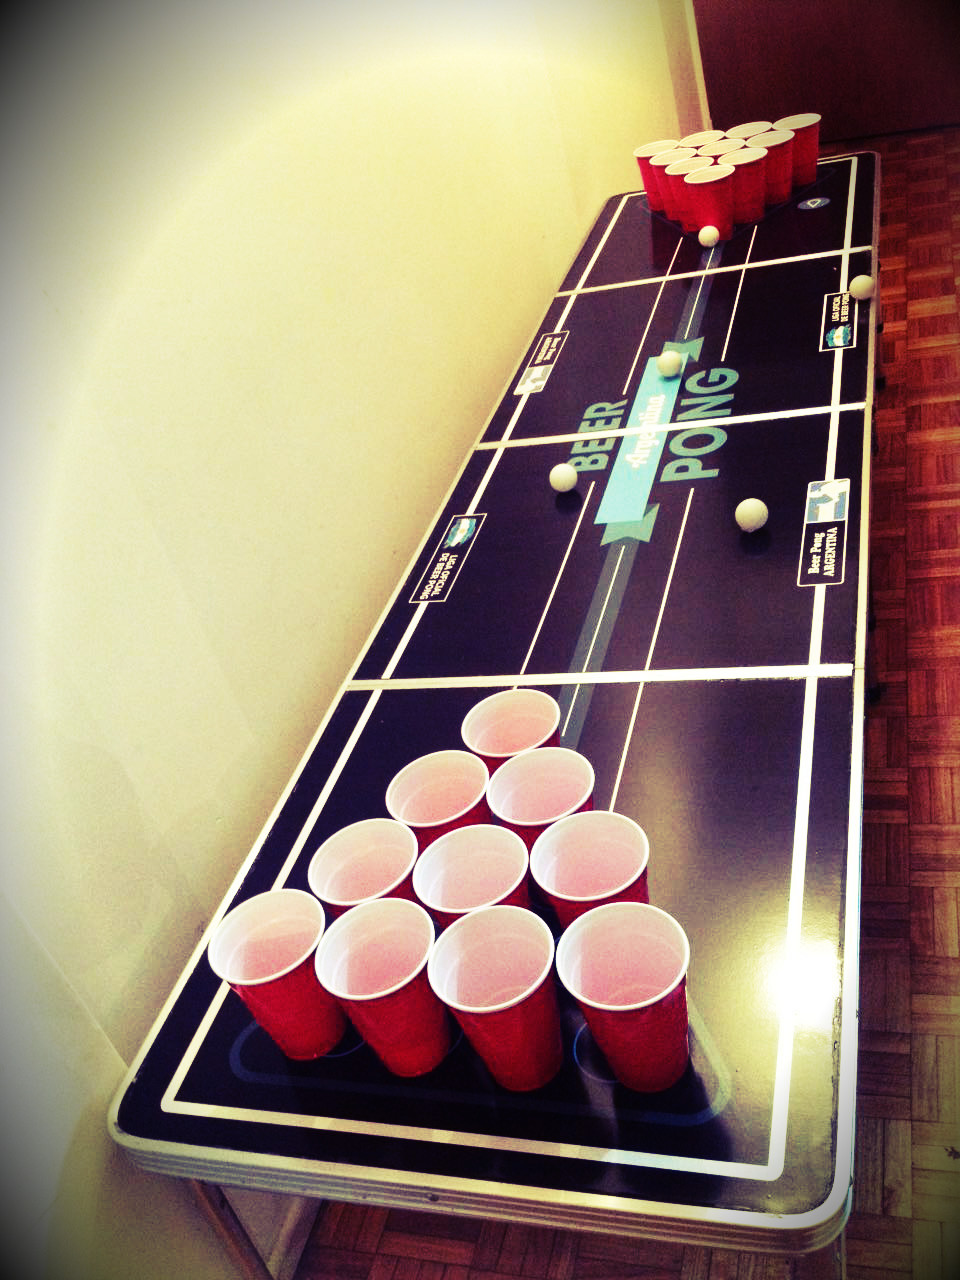
\includegraphics[width=0.7\linewidth]{beerpong}
	\caption{A typical setup of Beer Pong.}
	\label{beerpongsetup}
\end{figure}

At this party, when I first viewed the table of two players mid-game, one of the players had a strong lead, to wit she had significantly more cups on her side than her opponent. After making this initial observation, I moseyed into the kitchen to fix myself a drink. Upon my return, I found the score to be tied with one cup on either side of the table. I asked the player who was initially in the lead what had happened, and her response birthed the analysis before you. She answered my question with her own question: "Haven't you ever heard of choking?" What she had implied was that when there are a small number cups on the opponent's side, a psychological pressure affects the player's ability to perform well. The concept of "choking" under such pressure is very real and deep involving the idea of over-thinking as opposed to using the muscle memory developed from training and experience. Choking was certainly a possible explanation for the phenomenon which had occurred, but my hunch was of an orthogonal kind. I had figured that these types of games occur quite frequently due to the nature of random chance and probability, and not necessarily because a skilled player chokes at the end of a game. As the number of cups diminish on the opponent's side, so too does the probability of making a shot. This gives the opponent time to catch up and tie (or almost tie) the game at some point later. I posit the following hypothesis: there are significantly more games with large discrepancies in score at the beginning but \textit{small} discrepancies in score at the end than there are games with large discrepancies in score at the beginning and large discrepancies in score at the end due to random chance. To prove this, and to expose many other statistics of the game, I have written software that simulates playthroughs of Beer Pong. 

Keep in mind, a computer is not capable of choking. If, instead of simulations, a large number of real-life games were to be observed, and it was found that many games that started with large discrepancy scores ended with small discrepancy scores, then it would certainly support the idea of choking due to the fact that skills vary amongst players. However, if the skills of both players are equal and this phenomenon still occured then probability would be left as the only explanation. In other words, if the condition that one player is more skilled than another player is not implied then the phenomenon of a small discrepancy final score given a large discrepancy score near the beginning of the game would still occur more frequently than the phenomenon of a large discrepancy final score given a \textit{large} discrepancy score near the beginning of the game, and this phenomenon would be explained by randomness alone and not necessarily through a deterministic factor such as choking. 

\section{Design}
\subsection{Simulation}
\subsubsection{Differences and similarities between real-life games and simulated games}
The simulation has key differences between its design and a typical real-life game of Beer Pong. The differences do not hinder the confirmation or denial of the hypothesis that games frequently end in scores that are close to each other due to random chance and not necessarily any other exogenous sources. The first difference is that each player begins with 6 cups instead of 10. This was implemented for the sake of the speed of the simulation. Ten cups would theoretically not change the results that are germane to the hypothesis, but at least six cups are necessary due to the fact that the next largest amount is three cups wherein games that end in large discrepancy scores are virtually nonexistent. Another main difference is that players do not aim at cups in any way, the players make random shots at the opponent's cups. This makes the game purely probabilistic. This does not hinder the confirmation or denial of the hypothesis because although games in real life are not purely probabilistic, they are highly probabilistic. The reason being that the aim of players are not perfect due to lack of skill, and external forces unknown or for which are unaccounted by the player cause indeterministic fluctuations. A huge probabilistic component of the game is the fact that when there are more cups on the opponent's side, balls that were not headed straight for the inside of a cup sometimes bounce off of the rim of a cup and land in the cup or a nearby cup. This is one of the reasons that the probability of getting a ball in a cup when there are fewer cups diminishes. This component was incorporated into the design of the simulation.

Another difference between a real-life game and a simulated game is the game mechanic known as "re-racking." Many play Beer Pong with this rule, but it is absent in the simulation. This rule indicates that players at any point in the game may rearrange the cups on the opponent's side to the player's liking. Typically, players draw cups in closer to each other as removed cups have left space in between the remaining cups. This is usually allowed a maximum of twice per player per game. 

There were many other rules/mechanics in Beer Pong that were not incorporated into the simulation, with which some players play and some do not. The following is a non-exhaustive list of these:
\begin{itemize}
	\item If a player bounces a ball on the table during their turn and the ball lands in the opponent's cup, the opponent then removes a cup of the player's choosing in addition to the cup that had the ball land in it. However, if the player bounces the ball on the table, the opponent may swat the ball to prevent the shot from being made.
	\item If a ball spins around inside a cup, the opponent may blow the ball out of the cup or use their fingers to draw the ball out depending on whether the opponent is male or female, respectively.
	\item Players may play with two balls at a time instead of just one.
	\item Players may play two vs two. At parties, this is usually the case.
	\item Players may call in another player to substitute them for one turn. This is known as a "celebrity shot."
	\item If a ball bounces back to a player, the player may take another shot, but it must be from behind his/her back.
	\item In games of two vs two, if there is only one cup on the opponent's side both players on the opposite side must make the final shot in one round.
\end{itemize}

As mentioned earlier, a component of the game with probability built into its indeterministic nature was that a ball may hit the rim of a cup and land in the cup or a nearby cup. The simulation is designed such that if a ball hits the rim of a cup, it has an equal probability of bouncing one space left, right, forward, or back. This space may be a cup, slightly increasing the probability of making a shot.\footnote{or decreasing the probability depending on perspective.} Also, the game mechanic of a player going again on the condition that he/she made a shot was incorporated into the simulations. This was added in the interest of knowing whether or not going first played a significant role in the results of the games. 
\subsubsection{Mechanics of simulated games}
Both players start with a 9 $\times$ 9 grid on their side of the table. See Figure \ref{9x9grid}. Red circles represent 6 cups and their placement on the grid. The arrangement is viewed by a player on the opposite side of the table who would be the one to throw balls at this grid. The center of each grid square represents a point that a ball can hit each having probability of $\frac{1}{81}$ of being hit on any given throw of a ball. Each point is one of three possible types: "cup", "no cup", or "rim" represented by "c", "n", and "r", respectively in Figure \ref{points}. If a ball lands on a "no cup" square, it becomes the other player's turn to go. If it lands on a "rim" square, the ball randomly moves up, down, left, or right, each with a probability of $\frac{1}{4}$. The square it then bounces on may be any of the three types of squares.\footnote{In theory, the ball can bounce indefinitely since there are "rim" squares which are directly adjacent to one another.} Finally, if the ball lands on a "cup" square, the player goes again, the cup is removed, and the player earns a point.

\begin{figure}
	\centering
	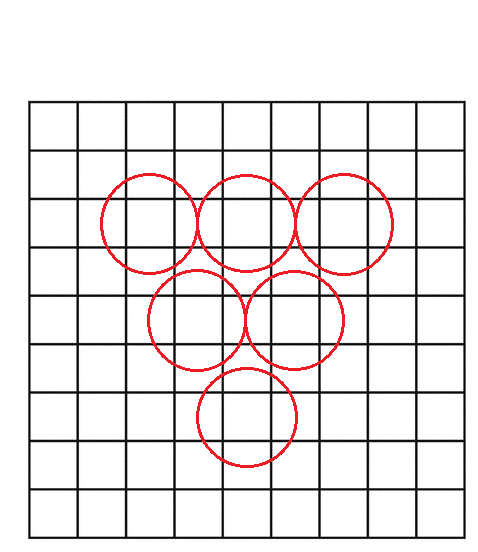
\includegraphics[width=0.7\linewidth]{gridwithcups}
	\caption{Theoretical arrangement of cups at the beginning of a game as viewed by a player on the opposite side.}
	\label{9x9grid}
\end{figure}

\begin{figure}
	\centering
	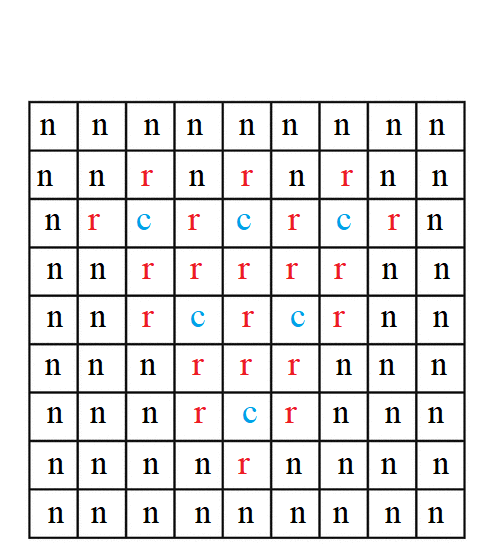
\includegraphics[width=0.7\linewidth]{gridwletters}
	\caption{Each player starts with an array of points labeled "n" (black), "r" (red), or "c" (blue), for "no cup," "rim," and "cup," respectively.}
	\label{points}
\end{figure}

When a cup is removed, the "cup" square changes to "no cup" as well as the "rim" squares above and below it, and sometimes to the left and right depending on which cup is removed and whether or not there is a cup to its left or right. The reason it depends on these conditions is because and right of one another share the same rim. For example, if the cup at the far left and very top were to be removed as in Figure \ref{cupremoval}, only the "rim" squares above, below, and to the left change to "no cup" squares because the cup to the right has not yet been removed and so it must keep its "rim" square. If for example, the very top cup in the center, i.e. the cup directly to the right of the cup that was just removed, was now removed, the "rim" square to its left may now be removed as seen in Figure \ref{2cupsremoved}.\footnote{Notice the "rim" square to its right remains since the cup to its right is still there.}

\begin{figure}
	\centering
	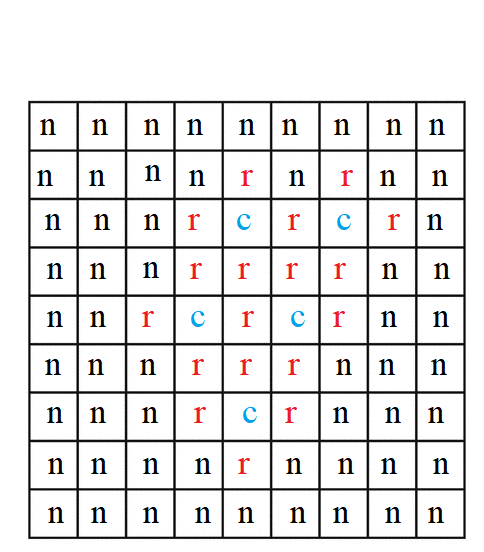
\includegraphics[width=0.7\linewidth]{cupremoval}
	\caption{The appearance of the opponent's array after only the top left cup has been removed.}
	\label{cupremoval}
\end{figure}

\begin{figure}
	\centering
	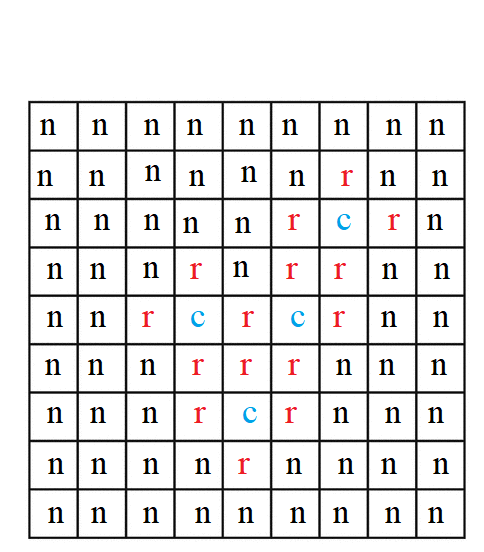
\includegraphics[width=0.7\linewidth]{2cupsremoved}
	\caption{The appearance of the opponent's array after the top left and the top center cup has been removed.}
	\label{2cupsremoved}
\end{figure}

The reader at this point may wonder about the size of the border surrounding the three cups. The border is necessary due to the fact that real-life players often miss the triangle of cups entirely. The size of the border is only one square because the players in the simulations are already not aiming at all, and so each game would take too long if the size were larger.

There are four types of shots that can be made. The first is hitting a rim of a cup, and then (eventually) landing the ball outside of any cup, i.e. into a "no cup" square. The next type of shot is directly into a "no cup" square, i.e. without hitting a rim first. The third type of shot is hitting a rim, and then (eventually) landing the ball inside a cup. The last type of shot is landing the ball directly inside a cup without first hitting the rim. In the interest of which types of shots were more common than others, the simulator keeps count of the types of shots in a single game.

\subsection{Software}
Understanding exactly how the software works and all of its logic is vital to adjudicating the validity of the simulation and veracity of the conclusions drawn from it.
\subsubsection{Libraries}
The code was written in Python 3 using Jupyter. The libraries used were "random" for random number generation and randomly choosing elements; "csv" to make comma separated value tables; "numpy" to make and view certain arrays, to dump them into csv files, to use mathematical functions such as log, and to add columns to dataframes; "pandas" for reading csv files; and "sklearn" to apply linear regression.
\begin{lstlisting}[language=Python]
import random
from random import randrange
import csv
import numpy as np
import pandas as pd
from sklearn import linear_model
\end{lstlisting}


\subsubsection{Setting up a game}
One of the functions written performs the simple job of creating an array for each player. The same function is used to set up the same array at the beginning of each game for both players producing identical setups. Some elements in the area were hard coded while some used loops to iterate through the array. Each element in the 9 $\times$ 9 grid was given a string value: "nocup", "cup", or "rim."
\begin{lstlisting}[language=Python]
def setUpPlayer():
    player1array = [[None for i in 
    range(9)] for j in range(9)]
    i = 0
    j =0
    for i in range(9):
        player1array[0][i] = "nocup"
        player1array[8][i] = "nocup"
        player1array[i][0] = "nocup"
        player1array[i][8] = "nocup"
    i=0

    for i in range(1,8,2):
        player1array[1][i] = 'nocup'
        player1array[2][i] = "rim"
    i=0

    for i in range(2,7,2):
    	player1array[1][i] = 'rim'
    	player1array[2][i] = 'cup'
    	player1array[4][i] = 'rim'
    i=0
    
    player1array[3][1] = 'nocup'
    player1array[3][7] = 'nocup'
    
    for i in range(2,7):
    	player1array[3][i] = 'rim'
    i=0
    
    player1array[4][1] = 'nocup'
    player1array[4][7] = 'nocup'
    player1array[4][3] = 'cup'
    player1array[4][5] = 'cup'
    player1array[5][1] = 'nocup'
    player1array[5][2]= 'nocup'
    player1array[5][6]= 'nocup'
    player1array[5][7]= 'nocup'
    
    for i in range(3,6):
    	player1array[5][i] = 'rim'
    i=0
    
    player1array[6][1]= 'nocup'
    player1array[6][2]= 'nocup'
    player1array[6][6]= 'nocup'
    player1array[6][7] = 'nocup'
    player1array[6][3] = 'rim'
    player1array[6][5] = 'rim'
    player1array[6][4] = 'cup'
    
    for i in range(1,4):
    	player1array[7][i] = 'nocup'
    i=0
    
    for i in range(5,8):
    	player1array[7][i] = 'nocup'
    i=0
    
    player1array[7][4] = 'rim'
    
    return player1array
\end{lstlisting}
\subsubsection{Playing 1 game}
The next function plays 1 Game of Beer Pong. The variable it takes in is either the integer number "1" or "2," indicating which player goes first. The function is designed to return many different values depending what kind of statistics were of interest. Many different return statements are written but only one is uncommented at a time.
\begin{lstlisting}[language=Python]
def play1Game(first2go):
\end{lstlisting}
The very first thing the function does is call the "setUpPlayer()" function to setup the two player arrays.
\begin{lstlisting}[language=Python]
player1array = setUpPlayer()
player2array = setUpPlayer()
\end{lstlisting}
The function checks who is the first to go and assigns a boolean value to a variable that is False if Player 1 goes first and True if Player 2 goes first. It then initializes several variables such as the score of each player before any balls are thrown, and how many times each type of shot was taken. These 11 variables\footnote{The 11 variables consist of the variable keeping track of whose turn it is, Player 1's array of cups, Player 2's array of cups, Player 1's score, Player 2's score, the number of times a shot hit a rim then missed, the number of times a shot did not hit a rim then missed, the number of times a shot hit the rim then made it into a cup, the number of times a shot did not hit the rim then made it into a cup, Player 1's score without Player 2, and Player 2's score without Player 1.} are passed along from this function to two other functions, to wit, the function that causes Player 1 to throw a ball towards Player 2 and vice versa. It then initializes the rounds, $t$, which acts as each game's global independent parameter, and $t_1$ and $t_2$ which acts as each player's local independent parameter. One increment in $t_1$ and $t_2$ is one more time that Player 1 and Player 2 throw the ball, respectively, while $t$ keeps track of how many times the ball was thrown by either player. The function also initializes integer versions of the quantities $t_1$ and $t_2$ with $j$ and $k$, respectively.
\begin{lstlisting}[language=Python]
if first2go == 1:
    player2turn = False
else:
    player2turn = True

player1score = [0]
player2score = [0]
player1scorelocal = [0]
player2scorelocal = [0]

rimthenmiss = 0
straightmiss = 0
rimthencup = 0
straightcup = 0

results = [player2turn, player1array, player2array,
player1score, player2score, 
rimthenmiss, straightmiss, rimthencup, straightcup,
player1scorelocal, 
player2scorelocal]
t = [0]
t1 = [0]
t2 = [0]
i=0
j=0
k=0
\end{lstlisting}

To play the game, the function performs a while loop which breaks if any one of the two players achieves a score of 6. Inside the while loop, the function calls the function of throwing a ball to the other player depending on whose turn it is. When it does so, it increases $t$ by 1, and keeps track of $j$ and $k$.
\begin{lstlisting}[language=Python]
while results[3][-1] < 6 and results[4][-1] < 6:
    if results[0] == True:
        results = player2throws(results)
        i += 1
        t.append(i)
		k += 1
		t2.append(k)
    else:
        results = player1throws(results)
	    i += 1
	    t.append(i)
	    j += 1
	    t1.append(j)
i=0
\end{lstlisting}

The player scores are non-Markovian stochastic processes of the random variable, $P_t$. As an approximation of a model, the non-homogeneous Poisson process was used although it is a Markovian model. As a non-homogeneous Poisson process, $P_t$ must contain a time varying intensity, $\lambda(t)$, which can be approximately found experimentally by simulations. To that end, the program checks for a jump in the points of Player 1 and records the time that the jump occurred. 
\begin{lstlisting}
throwsuntilpoint = []
for i in range(1,len(t1)):
    if results[9][i] > results[9][i-1]:
        throwsuntilpoint.append(t1[i])
i=0
\end{lstlisting}

The program keeps track of the score difference in two separate ways. The first way by subtracting Player 2's score from Player 1's score, while the second way is by taking the absolute value of the difference between the two scores. The former way indicates which player has the lead in that round. This method of calculating score differences is used in conjuction with the max and min operators to find which player had the biggest lead and during which round(s). The method that is not in use is simply commented out. If the "biggestlead" variable is a negative number, it means that Player 2 had the biggest lead at some point in the game. If the variable is a positive number, Player 1 had the biggest lead. If both players at one point in the game had the biggest lead, the variable "biggestlead" is assigned a value of 0.
\begin{lstlisting}[language=Python]
score_difference = [0]

for i in range(1,len(t)):
    score_difference.append(player1score[i] - \
    player2score[i])
i=0

for i in range(1,len(t)):
    score_difference.append(abs(player1score[i] - \
    player2score[i]))
i=0

if abs(min(score_difference)) > max(score_difference):
    biggestlead = min(score_difference)
elif abs(min(score_difference)) < max(score_difference):
    biggestlead = max(score_difference)
elif abs(min(score_difference)) == max(score_difference):
    biggestlead = 0
\end{lstlisting}

The program then checks which player is the winner by observing the final score of Player 1. It also stores $t$, Player 1's score, Player 2's score, and the score difference into an array and stores this array as a csv file. This was done for the purpose of observing the type of game that occurs wherein the variable "biggestlead" is assigned a value of 0. The program also dumps the numpy array of $P_t$ of Player 1 and $t_1$ which is the time parameter of $P_t$ into a csv file.

\begin{lstlisting}[language=Python]
if results[3][-1] == 6:
    winner = "Player 1"
else:
    winner = "Player 2"

a = np.array(np.transpose([t, results[3], results[4],
score_difference]))
np.savetxt("biggestlead0.csv", a, delimiter=",")

a = np.array(np.transpose([t1, results[9]]))
np.savetxt("P_t.csv", a, delimiter=",")
\end{lstlisting}

The function returns many variables as many different statistics were of interest. These were $P_t$ and its time, the number of times Player 2 threw the ball subtracted from the number of times Player 1 threw the ball, how many times the 4 different types of shots were taken divided by the total number of shots taken, the score difference at the final round, the Player who won, the total number of shots taken, the "biggestlead," the largest score difference using the second method to obtain it, the player score at each round\footnote{This is not to be confused with $P_t$. $P_t$ is the player score when only considering the score of 1 player, usually Player 1. The time of $P_t$ is not $t$, rather it is $t_1$ (or $t_2$). Therefore $P_t$ is not the player's score at each round, rather it is the score each time that player throws the ball. A "round" is a time at which \textit{any} player throws the ball.}, and the score difference at each round.

\begin{lstlisting}[language=Python]
return throwsuntilpoint
#return np.array([t1, results[9]])
#return j-k
#return [round(results[5]/t[-1],2),
#round(results[6]/t[-1],2), 
#round(results[7]/t[-1],2), round(results[8]/t[-1],2)]
#return score_difference[-1]    
#return winner
#return [t[-1],j-k,winner,score_difference[-1],results[5],
#results[6],results[7],
#results[8],biggestlead]
#return [max(score_difference), score_difference[-1]]
#return np.array([t, results[3], results[4], 
#score_difference, 
#max(score_difference)])
#return [biggestlead, winner]
#return np.array([biggestlead, winner, t, results[3], 
#results[4], 
#score_difference])
\end{lstlisting}

\subsubsection{Throwing the ball}
The 11 variables mentioned earlier get passed into these functions as a list of variables, each of which are given their own variable name. Before any player throws anything, the program assigns the value of False to the variable "rimhit" which states whether or not the ball hit a rim. It also keeps track of the score of the player is who not throwing the ball. Only the code in the function that has Player 1 throw to Player 2 is provided but the code that has Player 2 throw to Player 1 is identical but with all player variables reversed.
\begin{lstlisting}[language=Python]
def player1throws(results):
    player2turn = results[0]
    player1array = results[1]
    player2array = results[2]
    player1score = results[3]
    player2score = results[4]
    rimthenmiss = results[5]
    straightmiss = results[6]
    rimthencup = results[7]
    straightcup = results[8]
    player1scorelocal = results[9]
    player2scorelocal = results[10]

    rimhit = False
    player2score.append(player2score[-1])
\end{lstlisting} 

The player then chooses a random row and a random column of the opposing player's array and throws the ball at that position. If the ball hits a rim, the variable "rimhit" becomes True.
\begin{lstlisting}[language=Python]
row = randrange(len(player2array))
column = randrange(len(player2array))
hit = player2array[row][column]

if hit == "rim":
    rimhit = True
else:
    rimhit = False
\end{lstlisting} 

The ball is designed to keep repeating a certain action as long as it keeps hitting a rim and so those actions are all written under a while loop under that condition. A random number between 0 and 3 including 0 and 3 is generated and depending on which number was generated, the ball moves up, down, left, or right. In some circumstances, the ball hits another rim and stays in the while loop until it moves to a "cup" or a "nocup" square.

\begin{lstlisting}[language=Python]
while hit == "rim":
    n = randrange(4)
    if n == 0:
        column = column - 1
        hit = player2array[row][column]
    elif n == 1:
        row = row - 1
        hit = player2array[row][column]
    elif n == 2:
        column = column + 1
        hit = player2array[row][column]
    else:
        row = row + 1
        hit = player2array[row][column]
\end{lstlisting}

If the ball hits a "nocup", the code keeps track of whether the shot had hit a rim first or not, the Player's score, and whose turn it is. If the ball hits a "cup" square, the code keeps track of the same variables, making sure to add a point to the player's score, it then removes a cup. It does so by changing the "cup" square that had been hit to "nocup" as well as the "rim" squares that were below and above it. Then the program checks for exactly which cup had been hit and removed. Depending on which cup had \textit{just} been removed and which cups had \textit{already} been removed, the program changes the values of adjacent "rim" squares to "nocup" squares.

\begin{lstlisting}[language=Python]
if hit == "nocup":
    if rimhit == True:
        rimthenmiss += 1
    else:
        straightmiss += 1
    player1score.append(player1score[-1])
    player1scorelocal.append(player1scorelocal[-1])
    player2turn = True
if hit == "cup":
    if rimhit == True:
        rimthencup += 1
    else:
        straightcup += 1
    player1score.append(player1score[-1]+1)
    player1scorelocal.append(player1scorelocal[-1]+1)
    player2array[row][column] = "nocup"
    player2array[row-1][column] = "nocup"
    player2array[row+1][column] = "nocup"
    if row == 2 and column == 2:
        player2array[2][1] = "nocup"
        if player2array[2][4] == "nocup":
            player2array[2][3] = "nocup"
    if row == 2 and column == 4:
        if player2array[2][2] == "nocup":
            player2array[2][3] = "nocup"
        if player2array[2][6] == "nocup":
            player2array[2][5] = "nocup"
    if row == 2 and column == 6:
        player2array[2][7] = "nocup"
        if player2array[2][4] == "nocup":
            player2array[2][5] = "nocup"
    if row == 4 and column == 3:
        player2array[4][2] = "nocup"
        if player2array[4][5] == "nocup":
            player2array[4][3] = "nocup"
    if row == 4 and column == 5:
        player2array[4][6] = "nocup"
        if player2array[4][3] == "nocup":
            player2array[4][4] = "nocup"
    if row == 6 and column == 4:
        player2array[6][3] = "nocup"
        player2array[6][5] = "nocup"
\end{lstlisting}

Finally, it returns the 11 variables back to the function that plays 1 game.

\begin{lstlisting}[language=Python]
return [player2turn, player1array, player2array, 
player1score, player2score, rimthenmiss, straightmiss,
rimthencup, straightcup, player1scorelocal, 
player2scorelocal]
\end{lstlisting}

\subsubsection{Playing 1 set of many games}

This function takes an integer variable which tells it how many games to play and which player will go first. The statistics obtained from playing 1 game are usually averaged out here by playing many games. One of these statistics is the average number of times the winning player throws the ball until it scores. There are 6 different times for this since the player scores 6 times, and so these times are initiated as a list. The program was designed to play games of Beer Pong until there are 100 of these lists of 6 times, meaning the list becomes an array $100 \times 6$. The row of times is only added to the array if there are 6 of them.
The program then sums up each column of this array and divides each of the 6 sums by the number of games played to obtain the mean time of each score in a set of games.
\begin{lstlisting}[language=Python]
def playManyGames(games,first2go):

    lamdastime = []
    while len(lamdas) < games:
        results = play1Game(first2go)
        if len(results) == 7:
            lamdastime.append(results)

    summlamdastime = [0]*len(lamdastime[0])
    for i in range(len(lamdastime)):
        for j in range(len(lamdastime[i])):
            summlamdastime[j] = summlamdastime[j] + \
            lamdastime[i][j]
    i =0
    j=0

    meanlamdastime = []
    for i in range(len(summlamdastime)):
        meanlamdastime.append(summlamdastime[i]/\
        len(lamdastime))
    i=0
\end{lstlisting}

The function also obtains the statistics of how many times each type of shot was taken. When one game is played it produces a proportion of each type of shot and sends it to this function where it is stored until the desired number of games are played producing an expectation value for each proportion based on the number of times each proportion was observed.
\begin{lstlisting}[language=Python]
proportions = []
for i in range(games):
    results = play1Game(first2go)
    proportions.append(results)
i=0

array = np.array(proportions)
rimthenmisses = []
straightmisses = []
rimthenhits = []
straighthits = []
for i in range(len(proportions)):
    rimthenmisses.append(proportions[i][0])
    straightmisses.append(proportions[i][1])
    rimthenhits.append(proportions[i][2])
    straighthits.append(proportions[i][3])

rimthenmisses.sort()
straightmisses.sort()
rimthenhits.sort()
straighthits.sort()

rmdict = dict.fromkeys(rimthenmisses,0)
smdict = dict.fromkeys(straightmisses,0)
rhdict = dict.fromkeys(rimthenhits,0)
shdict = dict.fromkeys(straighthits,0)

for i in range(len(rimthenmisses)):
    rmdict[rimthenmisses[i]] += 1
    smdict[straightmisses[i]] += 1
    rhdict[rimthenhits[i]] += 1
    shdict[straighthits[i]] += 1

rmmean = 0
for rmkey in rmdict.keys():
    rmmean = rmmean + rmdict[rmkey]/games*rmkey
rhmean = 0
for rhkey in rhdict.keys():
    rhmean = rhmean + rhdict[rhkey]/games*rhkey
smmean = 0
for smkey in smdict.keys():
    smmean = smmean + smdict[smkey]/games*smkey
shmean = 0
for shkey in shdict.keys():
    shmean = shmean + shdict[shkey]/games*shkey
\end{lstlisting}

The function also keeps track of how many times a player won depending on which player went first in the interest of knowing whether or not the winner of a game is correlated with which player went first.
\begin{lstlisting}[language=Python]
player2count = 0
player1count = 0
for i in range(games):
    results = play1Game(first2go)
if results == "Player 2":
    player2count += 1
if results == "Player 1":
    player1count += 1
i=0
\end{lstlisting}

Overall there are three types of games that can occur: chokes, landslides, and neck and neck games.
Although the term "chokes" is used here they are not games where a computer "chokes" and feels human psychological pressure. They are games that appear to be chokes in the probabilistic sense. More specifically, they are games that start with high discrepancy scores but end with low discrepancy scores. The program constitutes games with maximum score differences at any point in the game larger than 3 and with final score differences smaller or equal to 3 as "chokes." The most obvious case of a "choke" is one player's score going from 0 to 5 points, achieving a max score difference of 5, then the other player going from 0 to 5 points, and then either player scoring the last point. This is considered a "choke" because at the last point, the player was not able to score before the other player caught up, which happens as a result of random chance. The least obvious case of a choke is the case where the scores of Player 1 and Player 2 (can be switched) behave in the following way:
\begin{enumerate}
	\item Player 1: 0 to 4 (achieves the maximum score difference necessary for the game to constitute as a "choke")
	\item Player 2: 0 to 1
	\item Player 1: 4 to 5
	\item Player 2: 1 to 3
	\item Player 1: 5 to 6 (achieves the final score difference necessary for the game to consitute as a "choke")
\end{enumerate}
This type of game has a maximum score difference of 4 (the minimum required for the condition to be satisfied) and a final score difference of 3 (the maximum allowed). However, even these extreme and rare cases are considered "chokes" because of no. 4 on the list. Player 1 allowed Player 2 to go from 1 to 3 points while Player 1 only had 1 more point left to win the game.

"Chokes," in a sense, are the opposite of "landslides." "Landslides," short for "landslide victories," are games which have a maximum score difference greater than 3 and final score differences greater than 3. The most obvious "landslides" are shutout games, i.e. games where one player scores 6 points and the other players does not score any. The least obvious "landslides" are games such as these:
\begin{enumerate}
	\item Player 1: 0 to 4 (achieves the maximum score difference necessary for the game to constitute as a "landslide")
	\item Player 2: 0 to 1
	\item Player 1: 4 to 5
	\item Player 2: 1 to 2
	\item Player 1: 5 to 6 (achieves the final score difference necessary for the game to constitute as a "landslide")
\end{enumerate}
This type of game has a maximum score difference of 4 (the minimum required for the condition to be satisfied) and a final score difference of 4 (the maximum allowed). This least obvious case looks similar to the least obvious case of a "choke." The only difference is in no. 4 where Player 2 did not score enough points for a spectator to observe a "choke." These two least obvious cases barely make the criteria for their type of game because they both resemble the third type of game, to wit, "necknecks," short for "neck and neck games."

"Necknecks" are games wherein the maximum score difference is less or equal to 3 and so is the final score. The most obvious case are games such as the following:
\begin{enumerate}
	\item Player 1: 0 to 1
	\item Player 2: 0 to 2
	\item Player 1: 2 to 3
	\item Player 2: 2 to 4
	\item Player 1: 3 to 5
	\item Player 2: 4 to 6
\end{enumerate}
In these types of games, the maximum score difference is 1 (which happened to alternate between both players at each step), and the final score difference was also 1. The least obvious case of a "neckneck" are games such as these:
\begin{enumerate}
	\item Player 1: 0 to 3
	\item Player 2: 0 to 1
	\item Player 1: 3 to 4
	\item Player 2: 1 to 2
	\item Player 1: 4 to 5
	\item Player 2: 2 to 3
	\item Player 1: 5 to 6
\end{enumerate}
In this game, Player 1 had a maximum score difference of 3 (the maximum allowed for the condition to be satisfied) and a final score difference of 3 (the maximum allowed). The hypothesis of the study states that the proportion of "chokes" is larger than the proportion of "landslides."
\begin{lstlisting}[language=Python]
chokes = 0
landslides = 0
neckneck = 0

for i in range(games):
    results = play1Game(1)
    if results[0] <= 3 and results[1] <= 3:
        neckneck += 1
    elif results[0] > 3 and results[1] <= 3:
        chokes += 1
    elif results[0] > 3 and results[1] > 3:
        landslides += 1
\end{lstlisting}

The types of games that are played may be categorized in a different way as well, i.e. into "surprises," "nosurprises," and "others." Games which are surprises are those where the "biggestlead" variable mentioned earlier is a negative number, but the winner turned out to be Player 1. It is a surprise because although it seemed that Player 2 was going to win the game, judging by the sign of the "biggestlead," Player 1 came out on top. Surprises also include games where the roles of Player 1 and Player 2 are reversed, i.e. games wherein the "biggestlead" is positive, but with Player 2 as the winner. There are of couse "nosurprises," where the sign of the "biggestlead" is in line with the winner. Finally, there are "others." These games are given to those where "biggestlead" was assigned a value of 0.
\begin{lstlisting}[language=Python]
surprises = 0
nosurprises = 0
others = 0
for i in range(games):
    results = play1Game(first2go)
    if results[0] < 0 and results[1] == "Player 1":
        surprises += 1
    elif results[0] < 0 and results[1] == "Player 2":
        nosurprises += 1
    elif results[0] > 0 and results[1] == "Player 1":
        nosurprises += 1
    elif results[0]  > 0 and results[1] == "Player 2":
        surprises += 1
    elif results[0] == 0:
        others += 1
\end{lstlisting}

Out of interest into what the average final score difference was, this function was also designed to find the average final score of a set of many games.
\begin{lstlisting}[language=Python]
finalscorelist = []
for i in range(games):
    results = play1Game(first2go)
    finalscorelist.append(results)
i=0
finalscorelist.sort()    
dictionary = dict.fromkeys(finalscorelist, 0)
for i in range(len(finalscorelist)):
    dictionary[finalscorelist[i]] += 1
i=0    

mean = 0
for key in dictionary.keys():
    mean = mean + dictionary[key]/games*key
\end{lstlisting}
The function returns all of these mean values for preparation to pass them along to a function which plays many sets of many games. It returns the mean values of the 6 times that scores are made. It returns means of the proportions of the four different types of shots that can be taken. Many of the means are rounded so as to produce a discrete distribution of several different values in the interest of observing the kind of distribution it would produce. The function also produces how many times a player won in 1 set of many games. It returned the proportions of games which were "surprises," "nosurprises," and "others" by dividing by the total number of games. It returns a similar set of proportions but for the other method of categorizing games, i.e. "chokes," "landslides," and "necknecks."
\begin{lstlisting}[language=Python]
return mean
#return meanlamdastime
#return [round(shmean,3),round(smmean,3),round(rhmean,3),
#round(rmmean,3)]
#return round(mean,1)
#return player2count
#return [surprises/games, nosurprises/games, 
#others/games]
#return [chokes/games, landslides/games, neckneck/games]
\end{lstlisting}

\subsubsection{Playing many sets of many games}
The function takes in as variables the number of sets of games to be played, the number of games to be played per set, and which player goes fist. This function essentially does the same thing every time it is used, but in sometimes different ways. In general, it stores the mean values obtained from playing 1 set of many games and plays another set of many games and stores that mean value. It stores many of these mean values from playing many sets of many games sometimes calculates the mean value from all the sets. Often times, the same code was used for several different statistics. 
\begin{lstlisting}[language=Python]
def playSetsofGames(sets,games,first2go):
\end{lstlisting}

A set of mean times when points were scored that one set of many games produced, are made many times. The mean of these sets are then calculated and used to find $\lambda(t)$ of $P_t$. The reason this code is different than the main code used in this function is because it involved an array of means as opposed to simply a list of means. It then found the mean of these means. It differs from the rest of the code in that the rest of the code does not find the mean of the means from playing many sets of many games, rather it produces distributions in the form of csv files where software such as Microsoft Excel was used to find mean values.
\begin{lstlisting}[language=Python]
lamdastime = []
for i in range(sets):
    results = playManyGames(games,first2go)
    lamdastime.append(results)
i=0

summlamdastime = [0]*len(lamdastime[0])
for i in range(len(lamdastime)):
    for j in range(len(lamdastime[i])):
        summlamdastime[j] = summlamdastime[j] + \
        lamdastime[i][j]
i =0
j=0

meanlamdastime = []
for i in range(len(summlamdastime)):
    meanlamdastime.append(summlamdastime[i]\
    /len(lamdastime))
i=0

lamdastime = np.array(meanlamdastime)
np.savetxt("lamda2oft.csv", lamdastime, delimiter=",")
\end{lstlisting}

Otherwise, the function used the same code over and over to produce distributions. Using a for loop, it stored the means from playing many games, many times into a list which was converted into a dictionary which counted how many times each mean showed up. The dictionaries were then dumped into csv files. The function had no need to return anything, but on occasion it was of interest to view the arrays or dictionaries there in Jupyter.
\begin{lstlisting}[language=Python]
meanlist = []
for i in range(sets):
    mean = playManyGames(games,first2go)
    meanlist.append(mean)
i=0
meanlist.sort()
dictionary = dict.fromkeys(meanlist,0)

for i in range(len(meanlist)):
    dictionary[meanlist[i]] += 1

with open('chokesproportions.csv', 'w') as f:
    for key in dictionary.keys():
        f.write("%s,%s\n"%(key,dictionary[key]))

return lamdastime
#return dictionary
\end{lstlisting}
\subsubsection{$\lambda(t)$}
The functions above revealed the expected intervals of time that $P_t$ increased by 1. Those times were 4.688, 10.6093, 18.1332, 28.2148, 43.1115, and 66.8165. Since \cite{geeks4geeeks}
\begin{equation}\label{m1}
E[P_t] = m(t) = \int_{0}^{t} \lambda(s)ds,
\end{equation}
\begin{align}\label{expectation}
\begin{split}
1 = \int_{0}^{4.688}\lambda(t)dt,
\\
1 = \int_{4.688}^{10.6093}\lambda(t)dt,
\\
1 = \int_{10.6093}^{18.1332}\lambda(t)dt,
\\
1 = \int_{18.1332}^{28.2148}\lambda(t)dt,
\\
1 = \int_{28.2148}^{43.1115}\lambda(t)dt, \text{ and}
\\
1 = \int_{43.1115}^{66.8165}\lambda(t)dt.
\end{split}
\end{align}
This suggests that what might work as an approximation to $\lambda(t)$ is the following:
\begin{equation}\label{lambda}
\lambda(t) = 
\begin{cases} 
1/(4.688) & 0 \leq t \leq 4.688 \\
1/(10.6093 - 4.688) & 4.688 < t \leq 10.6093 \\
1/(18.1332 - 10.6093) & 10.6093 < t \leq 18.1332 \\
1/(28.2148 - 18.1332) & 18.1332 < t \leq 28.2148 \\
1/(43.1115 - 28.2148) & 28.2148 < t \leq 43.1115 \\
1/(66.8165 - 43.1115) & 66.8165 < t \leq 66.8165. 
\end{cases}
\end{equation}
This function simply produces such an experimentally obtained $\lambda(t)$ and dumps it into a csv file so a more analytical lambda can be obtained using these values and linear regression.
\begin{lstlisting}[language=Python]
def lamdaoftime():
    t = np.linspace(0,66.8165,100)
    lamda = []
    for i in range(len(t)):
        if t[i] <= 4.688:
            lamda.append(1/4.688)
        if t[i] > 4.688 and t[i] <= 10.6093:
            lamda.append(1/(10.6093 - 4.688))
        if t[i] > 10.6093 and t[i] <= 18.1332:
            lamda.append(1/(18.1332 - 10.6093))
        if t[i] > 18.1332 and t[i] <= 28.2148:
            lamda.append(1/(28.2148 - 18.1332))
        if t[i] > 28.2148 and t[i] <= 43.1115:
            lamda.append(1/(43.1115 - 28.2148))
        if t[i] > 43.1115 and t[i] <= 66.8165:
            lamda.append(1/(66.8165 - 43.1115))
i=0

lamdaandtime = np.array(np.transpose([t, lamda]))
np.savetxt("experimentallamdaoft.csv", lamdaandtime, delimiter=",")

return lamdaandtime
\end{lstlisting}

\subsubsection{Linear regression}
It was assumed that $\lambda(t)$ takes on the form
\begin{equation}\label{lambda2}
\lambda(t) = Ce^{rt}.
\end{equation}
To find $C$ and $r$, linear regression was used by first using a different variable to linearize the model:
\begin{align}\label{expectation}
\begin{split}
z = log(\lambda) = log(Ce^{rt})
\\
= log(C) + log(e^{rt}).
\\
z = rt + b,
\end{split}
\end{align}
where
\begin{align}\label{bandc}
\begin{split}
b = log(C), \text{ meaning}
\\
C = e^b.
\end{split}
\end{align}
The linear regression function will return $r$ and $C$ by simply reading the csv file that is $\lambda(t)$, adding $z$ as a column, then using linear regression to find $r$ and $b$.
\begin{lstlisting}[language=Python]
def get_parameters(file_path):
    df = pd.read_csv(file_path)
    df['logoflambda'] = np.log(df['Lambda'])

    reg = linear_model.LinearRegression()
    reg.fit(df[['Time']],df['logoflambda'])

    return [reg.coef_, np.exp(reg.intercept_)]
\end{lstlisting}

The function returned 0.19048160756605725 as $C$ and -0.02731405 as $r$ making
\begin{equation}\label{lambda3}
\lambda(t) = 0.19048160756605725e^{-0.02731405t}.
\end{equation}
Substituting this into Eqn. \ref{m1} gives
\begin{equation}\label{m2}
E[P_t] = m(t) = -\frac{0.19048160756605725}{0.02731405}(e^{-0.02731405t} - 1)
\end{equation}
A function may then be made to create a csv file of the new $\lambda(t)$ as well as $m(t)$.

\begin{lstlisting}[language=Python]
def lamdaoftime2():
    t = np.linspace(0, 70, 100)
    lamda = []
    m = []
    for i in range(len(t)):
        lamda.append(0.19048160756605725*np.exp(
        -0.02731405*t[i]))
        m.append(0.19048160756605725/-0.02731405*(
        np.exp(-0.02731405*t[i]) - 1))
    i=0
    lamdasandtime = np.array(np.transpose([t, lamda]))
    mandt = np.array(np.transpose([t, m]))
    np.savetxt("lamdaoftanalytical.csv", lamdasandtime,
    delimiter=",")
    np.savetxt("expectationofNoft.csv", mandt, 
    delimiter=",")
    #return lamdasandtime
    return mandt
\end{lstlisting}
\subsubsection{$P(P_t = n)$}
A function can then be made to find the probability that $P_t = n$ for some time, $t$, or the number of times the winning player threw the ball. This probability is \cite{geeks4geeeks}
\begin{equation}\label{pr}
P(P_t = n) = \frac{[m(t)]^n}{n!}e^{-m(t)}.
\end{equation}
\begin{lstlisting}[language=Python]
def ProfNofteqn(n):
    t = np.linspace(0, 70, 1000)
    m = []
    P = []
    for i in range(len(t)):
        m.append(0.19048160756605725/-0.02731405*(
        np.exp(-0.02731405*t[i]) - 1))
        P.append(m[i]**n/factorial(n)*np.exp(-m[i]))
    i=0
    Pandt = np.array(np.transpose([t,P]))
    np.savetxt("ProfNofteq6.csv", Pandt, delimiter=",")

    return Pandt
\end{lstlisting}
\section{Results}
\subsection{Significance of going first}
It is of interest to know whether or not throwing the ball first works in favor or against the player that does it. When Player 1 goes first, the distribution of the proportions of games won by Player 1 is seen in Fig. \ref{1wins1goesfirst}. The ordinate represents the number of sets of games which produced the corresponding proportion on the abscissa. Each set produced a proportion from 100 games, with 100 sets in total. The distribution in Fig. \ref{1wins1goesfirst} had a mean of about $\hat{p} = 0.51$ with a standard error of about $SE_{\hat{p}} = 0.049$. This means there is about a $95\%$ probability that the true proportion of games won by Player 1 with Player 1 going first lies in between $0.41$ and $0.61$.
\begin{figure}
	\centering
	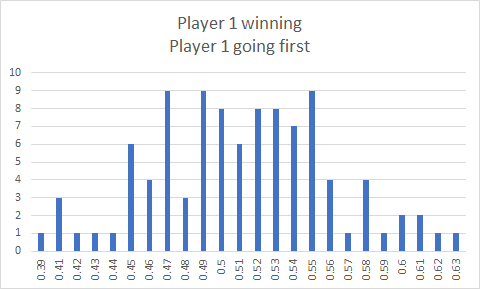
\includegraphics[width=0.7\linewidth]{1wins1goesfirst}
	\caption{A distribution of the proportion of games won by Player 1 with Player 1 going first every time. $\hat{p} = 0.51 \pm 0.099$, $SE_{\hat{p}} = 0.049$.}
	\label{1wins1goesfirst}
\end{figure}

When Player 1 goes first, the distribution of the proportions of games won by Player 2 is seen in Fig. \ref{2wins1goesfirst}. The distribution had a mean of about $\hat{p} = 0.50$ with a standard error of about $SE_{\hat{p}} = 0.053$. This means there is about a $95\%$ probability that the true proportion of games won by Player 2 with Player 1 going first lies in between $0.39$ and $0.61$.
\begin{figure}
	\centering
	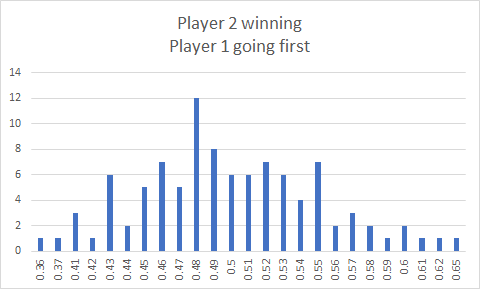
\includegraphics[width=0.7\linewidth]{2wins1goesfirst}
	\caption{A distribution of the proportion of games won by Player 2 with Player 1 going first every time. $\hat{p} = 0.50 \pm 0.106$, $SE_{\hat{p}} = 0.053$.}
	\label{2wins1goesfirst}
\end{figure}

When Player 2 goes first, the distribution of the proportions of games won by Player 1 is seen in Fig. \ref{1wins2goesfirst}. The distribution had a mean of about $\hat{p} = 0.49$ with a standard error of about $SE_{\hat{p}} = 0.044$. This means there is about a $95\%$ probability that the true proportion of games won by Player 1 with Player 2 going first lies in between $0.40$ and $0.58$.
\begin{figure}
	\centering
	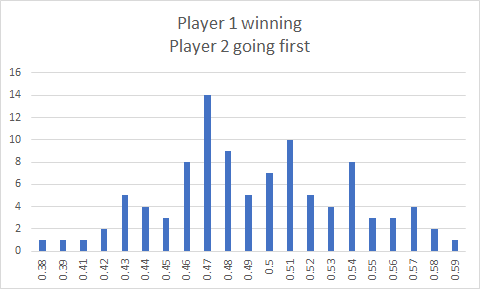
\includegraphics[width=0.7\linewidth]{1wins2goesfirst}
	\caption{A distribution of the proportion of games won by Player 1 with Player 2 going first every time. $\hat{p} = 0.49 \pm 0.089$, $SE_{\hat{p}} = 0.044$.}
	\label{1wins2goesfirst}
\end{figure}

When Player 2 goes first, the distribution of the proportions of games won by Player 2 is seen in Fig. \ref{2wins2goesfirst}. The distribution had a mean of about $\hat{p} = 0.50$ with a standard error of about $SE_{\hat{p}} = 0.055$. This means there is about a $95\%$ probability that the true proportion of games won by Player 2 with Player 2 going first lies in between $0.39$ and $0.61$.
\begin{figure}
	\centering
	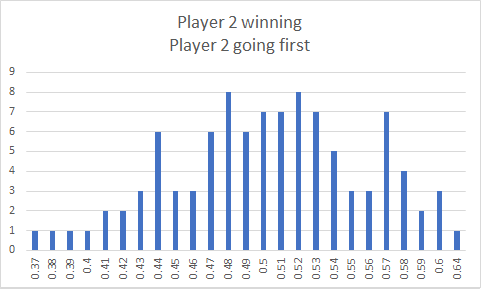
\includegraphics[width=0.7\linewidth]{2wins2goesfirst}
	\caption{A distribution of the proportion of games won by Player 2 with Player 2 going first every time. $\hat{p} = 0.50 \pm 0.110$, $SE_{\hat{p}} = 0.055$.}
	\label{2wins2goesfirst}
\end{figure}

To further examine the significance of going first, the value
\begin{equation}\label{delta}
\Delta = j - k
\end{equation}
was observed, where $j$ is the number of times Player 1 threw the ball and $k$ is the number of times Player 2 threw the ball in a single game. When Player 1 went first, the distribution of the mean value of $\Delta$ is seen in Fig. \ref{delta1goesfirst}. The mean value is about $\hat{\mu} = 0.5$ with a standard error of about $SE_{\hat{\mu}} = 0.14$, meaning there is a $95\%$ probability that the true mean, $\mu$ lies in between $0.2$ and $0.8$.

\begin{figure}
	\centering
	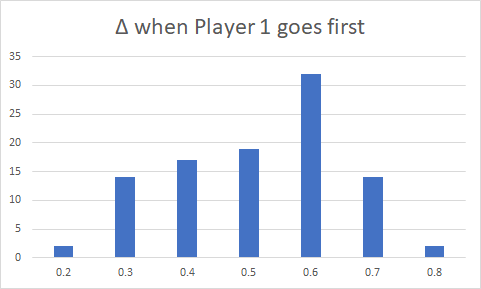
\includegraphics[width=0.7\linewidth]{delta1goesfirst}
	\caption{A distribution of $\Delta$ with Player 1 going first every time. $\hat{\mu} = 0.5 \pm 0.28$, $SE_{\hat{p}} = 0.14$.}
	\label{delta1goesfirst}
\end{figure}

When Player 2 went first, the distribution of the mean value of $\Delta$ is seen in Fig. \ref{delta2goesfirst}. The mean value is about $\hat{\mu} = -0.5$ with a standard error of about $SE_{\hat{\mu}} = 0.16$, meaning there is a $95\%$ probability that the true mean, $\mu$ lies in between $-0.2$ and $-0.8$.

\begin{figure}
	\centering
	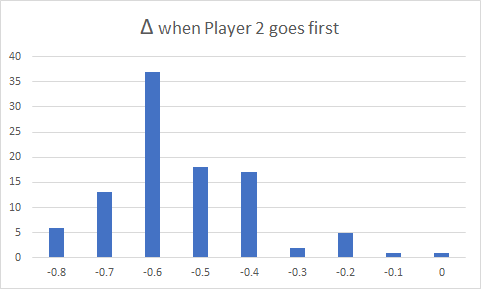
\includegraphics[width=0.7\linewidth]{delta2goesfirst}
	\caption{A distribution of $\Delta$ with Player 2 going first every time. $\hat{\mu} = -0.5 \pm 0.31$, $SE_{\hat{p}} = 0.16$.}
	\label{delta2goesfirst}
\end{figure}

Each game must have an odd or an even number of throws, which means for the games with an odd number of throws, which is probably about half, there must be a player with at least 1 more throw than the other. The results suggest that about half of the games that have Player 1 going first, end with Player 1 having 1 more throw than Player 2, and vice versa, while the other half of games end with the two players having the same amount of throws. This is not actually what happens every time, but it is essentially a summary.

It is inconclusive if going first plays any contribution to winning a game of Beer Pong. As a consequence, most of the statistics gathered in the remainder of the paper were gathered from simulations of games without regard to which player went first.

\subsection{Differences in final scores}
The distribution of final scores were also of interest because it may provide insight into the hypothesis of the paper. The distribution of mean differences in final scores over 100 sets of 100 games in each set is seen in Fig. \ref{finalscores}. The ordinate shows the number of sets of games which produced the corresponding mean absolute difference in the scores of the two players on the very last round in the abscissa. The mean of the distribution was about $\hat{\mu} = 1.62$ with a standard error of about $SE_{\hat{\mu}} = 0.082$. This means that there is a about $95\%$ probability that the true mean, $\mu$, lies somewhere between $1.45$ and $1.79$.

\begin{figure}
	\centering
	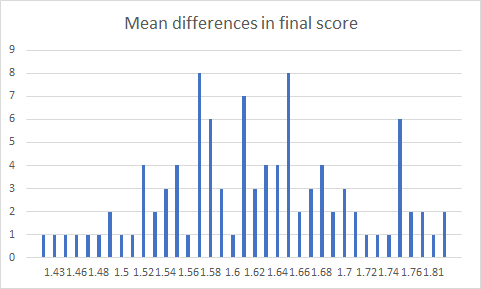
\includegraphics[width=0.7\linewidth]{finalscores}
	\caption{A distribution of the means of absolute differences in scores on the final round of games. $\hat{\mu} = 1.62 \pm 0.164$, $SE_{\hat{p}} = 0.082$.}
	\label{finalscores}
\end{figure}

The results show that a typical (simulated) game of Beer Pong ends with the winning player having about 1 to 2 cups more than the losing player. Assuming a spectator had only this data to reference, after observing the beginning of a real-life game where the player in the lead still had much more cups on his/her side than his/her opponent, the safest bet to make on the amount of cups with which that player ends the game is about 2.

\subsection{Types of shots}

Each game had a different total number of throws, and each throw was one of four different types discussed earlier. The four types of shots are hitting a rim or rims then landing the ball inside a cup, landing the ball inside a cup without hitting any rims, hitting a rim or rims then missing any cup, and missing any cup without hitting any rim. It was of interest to know which types of shots were more popular than others. When the simulation played 1 game, a proportion of each type was calculated by dividing the number of times each type of shot was taken by the total number of shots taken in that game. This produced four different proportions for each game. One set of games consisted of 100 games and produced one mean proportion for each type of shot out of the 100 games. The program simulated 100 sets of 100 games to find the mean value of these 100 means of these proportions. The results of the 100 sets of games are summarized by Fig. \ref{typesofshots}.

\begin{figure}
	\centering
	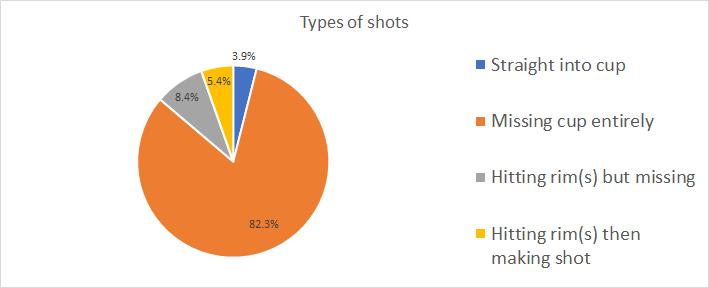
\includegraphics[width=0.7\linewidth]{typesofshots}
	\caption{The proportions of the different types of shots possible in a game of Beer Pong.}
	\label{typesofshots}
\end{figure}

The results reflect proportions of games in general and do not necessarily reflect probabilities of these occurances at given times in each game. They show, e.g., that overall, if a ball hit a rim, it will most likely not go into a cup. This statement however might be untrue at different times of the game. The results show that, overall, the probability of making a shot was about $9.3\%$ while the probability of missing was $90.7\%$.

\subsection{Types of games}
Recalling from the previous section, there were two ways to categorize types of games. The two ways are grouped and labeled as "Types of Games I," and "Types of Games II." 
\subsubsection{Types of Games I: Chokes, landslide victories, and neck and neck matches}
Types of Games I consists of "chokes," "landslides," and "necknecks." Although the term "choke" is used, it is merely used as a way to categorize games that would \textit{appear} to have a player suffering from the psychological effect known as "choking." In fact, one of the purposes of the paper is to show that games often appear to be ones where a player chokes, but it might be simply a result of randomness. 

How a game is categorized depends on what the absolute value of the maximum score difference was in the game, and the absolute value of the final score difference.\footnote{Refer to Section 2.2.5.} It is of interest to know the proportion of games which had the player with a massive lead allow the opponent to catch up before the end of the game, the proportion of games which had the player with a massive lead win the game, and the proportion of games where there simply was no massive lead. The results of these statistics are shown in Fig. \ref{typesofgames1}.

\begin{figure}
	\centering
	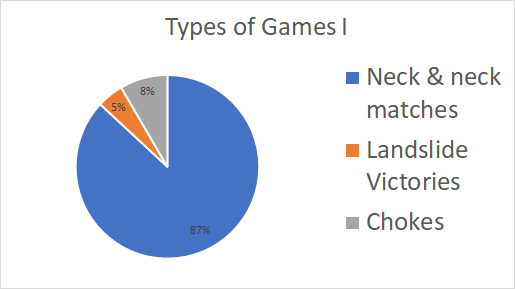
\includegraphics[width=0.7\linewidth]{typesofgames1}
	\caption{The proportions of the different types of games possible in a game of Beer Pong. These types are of the Types of Games I group.}
	\label{typesofgames1}
\end{figure}

The results indicate the probability of what type of game will occur before the game starts at all. However, if one were to make an observation of a game mid-game and found that one player had a massive lead on another, the probability that the game consists of what would appear to be a choke is higher than the probability of the game ending with the player with the massive lead maintaining his/her massive lead, thus confirming the hypothesis.

\subsubsection{Types of Games II: surprises, no surprises, and others.}

The second way to categorize games are by "surprises," "nosurprises," and "others." Those depend on which player had the largest lead during the game and which player was the winner. See section 2.2.5 for more details. A surprising game, i.e. a "surprise," is one where the player with the largest lead in the game is not the player who won the game. A game which is not surprising, i.e. a "nosurprise," is just the opposite. However, if both players had the largest lead at some point in the game, it constitutes as an "other." A typical "other" game is demonstrated in Table \ref{other}. Notice that both players had the largest lead at some point in the game, to wit, winning by two points. It is not possible for both players to have a lead on the other that is greater than three points. For that reason, "others" are a subset of "necknecks." 
\begin{table}[h!]
	\centering
	\begin{tabular}{||c c c c||} 
		\hline
		$t$ & $P_{1t}$ & $P_{2t}$ & $P_{1t} - P_{2t}$ \\ [0.5ex] 
		\hline\hline
		0 & 0 & 0 & 0 \\
		1 & 1 & 0 & 1 \\ 
		2 & 2 & 0 & 2 \\
		3 & 2 & 0 & 2 \\
		4 & 2 & 1 & 1 \\
		5 & 2 & 1 & 1 \\
		6 & 2 & 1 & 1 \\ 
		7 & 2 & 1 & 1 \\
		8 & 2 & 1 & 1 \\
		9 & 2 & 1 & 1 \\
		10 & 2 & 1 & 1 \\
		11 & 2 & 2 & 0 \\ 
		12 & 2 & 2 & 0 \\
		13 & 3 & 2 & 1 \\
		14 & 3 & 2 & 1 \\
		15 & 3 & 2 & 1 \\
		16 & 3 & 2 & 1 \\ 
		17 & 3 & 2 & 1 \\
		18 & 3 & 2 & 0 \\
		19 & 3 & 3 & 0 \\
		20 & 3 & 4 & -1 \\
		21 & 3 & 4 & -1 \\ 
		22 & 3 & 4 & -1 \\
		23 & 3 & 4 & -1 \\
		24 & 4 & 4 & -1 \\
		25 & 4 & 4 & -1 \\
		26 & 4 & 4 & 0 \\ 
		27 & 4 & 4 & 0 \\
		28 & 4 & 4 & 0 \\
		29 & 4 & 4 & 0 \\
		30 & 4 & 5 & -1 \\
		31 & 4 & 5 & -1 \\ 
		32 & 4 & 5 & -1 \\
		33 & 4 & 6 & -2 \\ [1ex] 
		\hline
	\end{tabular}
	\caption{A typical "other" game. $P_{1t}$ represents the score of Player 1 at time, t. Likewise $P_{2t}$ represents the score of Player 2 at time, t.}
	\label{other}
\end{table}

Fig. \ref{typesofgames2} shows the proportions of the types of games that occur. Note, the proportions do not add to 100\% because they are mean values collected from samples and are not necessarily the true proportions, but vary from the true proportions slightly.

\begin{figure}
	\centering
	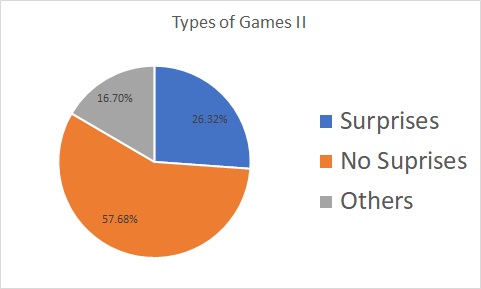
\includegraphics[width=0.7\linewidth]{typesofgames2}
	\caption{The proportions of the different types of games possible in a game of Beer Pong. These types are of the Types of Games II group.}
	\label{typesofgames2}
\end{figure}

\subsection{$P_t$}

$P_t$ is the stochastic random variable defined as the number of points a given player has as a function of the number of times that player has thrown the ball, $t$\footnote{This $t$ is not the same as the more global $t$ which includes the throws of both players.}. It is non-Markovian in nature since the probability of scoring a point depends on how many points have already been scored due to the removal of cups. However, a non-homogeneous Poisson process may be used as a model since the the process contains occasional jumps of unity value whose frequency tends to decrease with time, thus having a time varying intensity, $\lambda(t)$. A typical trajectory of $P_t$ is shown in Fig. \ref{P_t}. The interval of time $[33, 67]$ can be interpreted as a typical period of "choking."

\begin{figure}
	\centering
	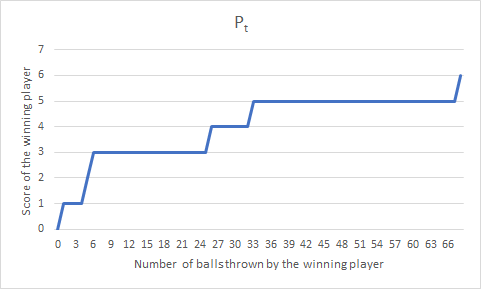
\includegraphics[width=0.7\linewidth]{P_t}
	\caption{A typical trajectory of the non-homogeneous Poisson process, $P_t$.}
	\label{P_t}
\end{figure}

As discussed in Section 2.2.7, the $P_t$ was expected to increase by 1 point during certain time intervals. Those time intervals were from 0 to 4.688, 10.6093, 18.1332, 28.2148, 43.1115, and 66.8165. One game of simulated Beer Pong revealed a set of six times. Playing 100 simulations revealed a set of 6 mean values of 100 sets of times. Playing 100 sets of 100 games revealed 100 sets of 6 mean values of times each set. Taking the mean values of these 100 sets produced the 6 mean values of times above. Using Eqns. \ref{m1} and \ref{expectation}, an experimentally found $\lambda(t)$ was found to be that of Eqn. \ref{lambda}. Fig. \ref{experimentallambda} shows a plot of this $\lambda(t)$. 

\begin{figure}
	\centering
	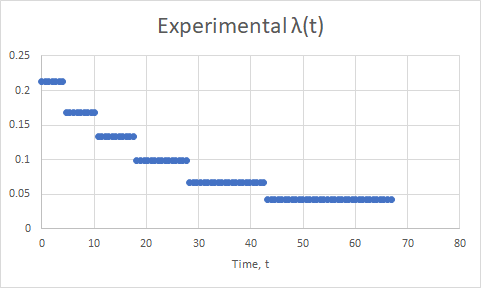
\includegraphics[width=0.7\linewidth]{experimentallambda}
	\caption{The experimentally found $\lambda(t)$.}
	\label{experimentallambda}
\end{figure}

Linear regression may be used to turn this function into a smooth function of time, Eqn. \ref{lambda3}. A plot of that $\lambda(t)$ is seen in Fig. \ref{smoothlambda}.

\begin{figure}
	\centering
	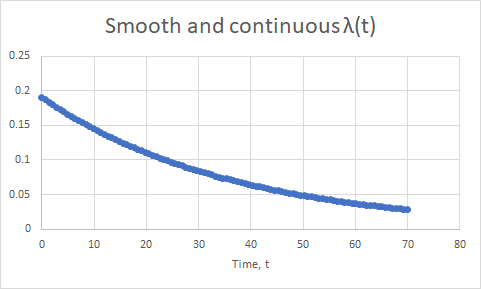
\includegraphics[width=0.7\linewidth]{smoothlambda}
	\caption{The experimentally found $\lambda(t)$ converted into a smooth function, $\lambda(t) = 0.19048160756605725e^{-0.02731405t}$.}
	\label{smoothlambda}
\end{figure}

Using Eqn. \ref{m1}, the expectation value of $P_t$, i.e. $m(t)$ was found. This $m(t)$ indicates how many points a player is expected to have as a function of the number of times that player has thrown the ball, and is shown in Fig. \ref{m}.

\begin{figure}
	\centering
	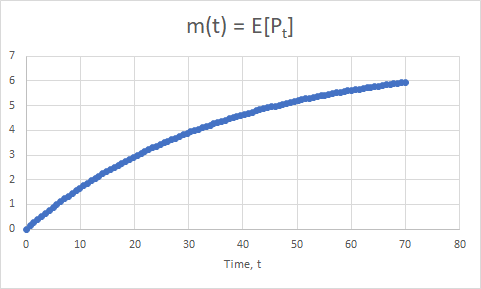
\includegraphics[width=0.7\linewidth]{m}
	\caption{The expected number of points a player will earn as a function of the number of times that player throws the ball, $E[P_t] = m(t) = -\frac{0.19048160756605725}{0.02731405}(e^{-0.02731405t} - 1)$.}
	\label{m}
\end{figure}

Substituting Eqn. \ref{m2} into Eqn. \ref{pr} gives 6 different probability distributions, $P(P_t = n)$ for $n = 1, 2, 3, 4, 5,$ and $6$. Those six probability distributions are depicted in Fig. \ref{PofPteqn}. Note that the six figures illustrate probability distributions and not probability \textit{density} functions. Therefore, the probability itself is on the ordinate and not to be taken as the integral over an interval of time of one of the functions. Each probability distribution aligns with intuition when examined closely. For example, looking at Fig. \ref{PofPteq1}, the probability that the first point is made within the first 5 throws is much higher than after. That is because after that, the player is more likely to score the second point, or third, etc. 

\begin{figure}
	\begin{subfigure}{.5\textwidth}
		\centering
		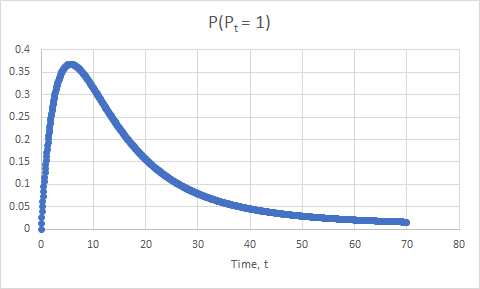
\includegraphics[width=.8\linewidth]{PofPteq1}
		\caption{$n = 1$}
		\label{PofPteq1}
	\end{subfigure}
	\begin{subfigure}{.5\textwidth}
		\centering
		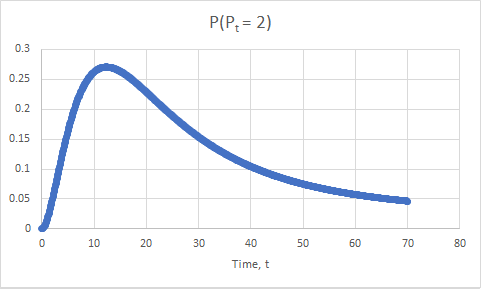
\includegraphics[width=.8\linewidth]{PofPteq2}
		\caption{$n = 2$}
		\label{PofPteq2}
	\end{subfigure}
	\begin{subfigure}{.5\textwidth}
		\centering
		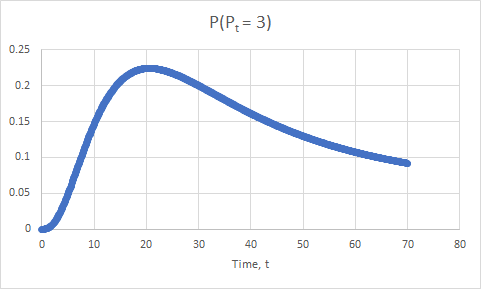
\includegraphics[width=.8\linewidth]{PofPteq3}
		\caption{$n = 3$}
		\label{PofPteq3}
	\end{subfigure}
	\begin{subfigure}{.5\textwidth}
		\centering
		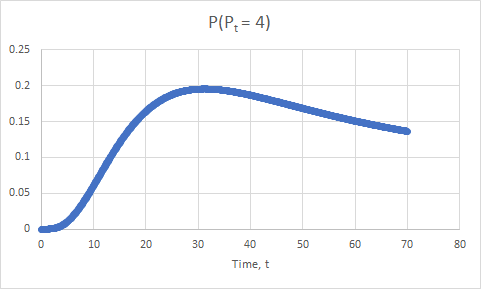
\includegraphics[width=.8\linewidth]{PofPteq4}
		\caption{$n = 4$}
		\label{PofPteq4}
	\end{subfigure}
	\begin{subfigure}{.5\textwidth}
		\centering
		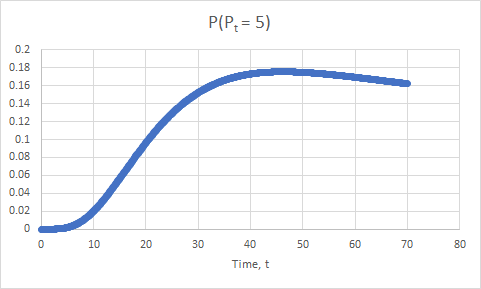
\includegraphics[width=.8\linewidth]{PofPteq5}
		\caption{$n = 5$}
		\label{PofPteq5}
	\end{subfigure}
	\begin{subfigure}{.5\textwidth}
		\centering
		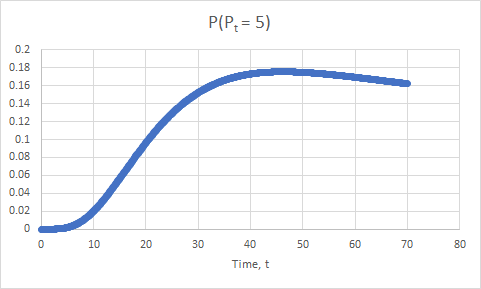
\includegraphics[width=.8\linewidth]{PofPteq5}
		\caption{$n = 6$}
		\label{PofPteq6}
	\end{subfigure}
	\caption{Probability distributions, $P(P_t = n)$ for each $n$.}
\label{PofPteqn}
\end{figure}

\section{Conclusion}
\subsection{General remarks}
The psychological phenomenon of choking may certainly play a contribution to the higher frequency of games of Beer Pong which consist of small final score discrepancies and large initial score discrepancies than large final score discrepancies and large initial score discrepancies. However, the results of this work suggest that this difference in frequencies need not any psychological effects for its existence. What happened on the day of the ugly sweater party happened because the probability of maing a shot decreases as the number of cups on the opponents side diminishes. That is a simple consequence of the fact that the probability space changes. The probability, while not directly related to the number of cups available on the opponenent's side, is correlated due to the sheer fact that
\begin{equation}\label{sheerprob}
\frac{\text{number of "cup" squares}}{\text{number of "cup" squares} + \text{number of "nocup" squares}}
\end{equation}
diminishes. 
It is also highly dependent on the location of the cups and whether or not the cups are near each other. The reason is due to the phenomenon of hitting rims of cups. The simulation may have placed a higher probability of landing a ball into a cup after hitting a rim than in real life, but this high probability may as well be compensated by the fact that real people aim. Aiming brings the ball to the general location of the group of cups that are aggregated without necessarily landing the ball in the exactly desired position.

The probability of the outcome of a game is contigent upon information contained in the set, $I_t$, already gathered about the game. In the case of the observation made at the ugly sweater party, the score at some point in the game, i.e. $P_t$ of both players was $I_t$-adapted. According to the simulations, the probability that the game ends in a small discrepancy score is very high. However, once it was observed that at some time, $t$, there was a large discrepancy in the points, that information became $I_t$-adapted. The probability that the game ends in a small discrepancy score is therefore shifted from $95\%$\footnote{$\frac{\text{"chokes"} + \text{"necknecks"}}{\text{total}}$} to $62\%$\footnote{$\frac{\text{"chokes"}}{\text{"chokes"} + \text{"landslides"}}$}, according to the results of Section 3.4.2. Having said that, there is still a larger probability that the game will end in a small discrepancy score than a large one. The probability of a "choke" is small, but once it is learned that a "neckneck" match is not possible, the probability of a "choke" changes dramatically (from $8\%$ to $62\%$).

The $\lambda(t)$ that speaks on all of the statistics of $P_t$ was obtained experimentally from the simulations, but varies from person to person in real life. However, the general principle, i.e. the shape and general form of $\lambda(t)$ may be the same for all players. To obtain a real $\lambda(t)$, $m(t)$, and $P(P_t = n)$, the $\lambda(t)$ in Fig. \ref{smoothlambda} may simply have to be scaled to fit the typical number times the real-life player in question throws the ball. In other words, the constants, $C$ and $r$ will have to change, but the general form, i.e. Eqn. \ref{lambda2} stays.

\subsection{Suggestions for further research}
The simulation has a lot of room for modification. For example, it would be interesting to know how the results compare if there were teams playing and some if not all of the team rules were applied such as two balls being thrown, the fact that both members of the team have to score the last point in the same round\footnote{This rule especially would cause an inflation in the proportion of games that end in small discrepancy final scores.}, etc. 

It is also of interest to extrapolate the statistics gathered to higher numbers of cups without altering the simulation's algorithm. Because $P_t$ is non-Markovian, the $\lambda(t)$, $m(t)$, and $P(P_t = n)$ obtained from simulating the game with 6 cups does not extend to 10 cups or more. The coefficients, $C$ and $r$ would be different, but the general form of $\lambda(t)$ would be the same. The coefficients used for 6 cups would not be extended to n cups because of an essential assumption made when using the Poisson process, whether it be homogeneous or non-homogeneous. That assumption is that "the numbers of events that occur in disjoint time intervals are independent." \cite{georgesbook} It might be possible, however, to find a $C(n)$ and an $r(n)$ in order to generalize the model to $n$ cups.

It would also be interesting to explore the properties of the difference in scores between two players, $P_{1t} - P_{2t}$. The two stochastic processes presumably have equivalent intensities, $\lambda(t)$, and thus their difference must be a martingale \cite{neftci} which would reveal several predictive measures.  

\bibliographystyle{unsrt}
\bibliography{references}

\end{document}